\documentclass[pdflatex,sn-mathphys-num]{sn-jnl}

\usepackage{graphicx}
\graphicspath{{../Images/}}
\usepackage{amsmath}
\usepackage{amssymb}
\usepackage{booktabs}
\usepackage{multirow}
\usepackage{hyperref}
\usepackage{algorithm}
\usepackage{algorithmicx}
\usepackage{algpseudocode}

\begin{document}

\title[Multi-Task Spectral Transformers for Sapota Quality]{Quantifying Sugar and Carbohydrate Levels in Sapota Using Hyperspectral Imaging and Multi-Task Spectral Transformers}

\author*[1]{\fnm{Swati} \sur{Hira}}\email{shira@iiitn.ac.in}
\author[1]{\fnm{Devguru} \sur{Tiwari}}\email{bt23csd060@iiitn.ac.in}

\affil*[1]{\orgdiv{Department of Computer Science and Engineering}, \orgname{Indian Institute of Information Technology Nagpur}, \city{Nagpur}, \state{Maharashtra}, \country{India}}

\abstract{The non-destructive evaluation of internal biochemical properties in fruits is a fundamental challenge in precision agriculture. While fruits with distinct visual ripening cues can be assessed using standard machine vision, fruits such as Sapota (\textit{Manilkara zapota}), which exhibit negligible external color changes during senescence, require advanced chemical analysis to accurately predict readiness for consumption. Traditional non-destructive chemometric methods often rely on shallow feature extraction and struggle against the high dimensionality of hyperspectral data, known as the Hughes phenomenon \cite{gowen2007hyperspectral, paoletti2019deep}. In this study, we propose a multi-task spectral Transformer architecture: the Multi-Task Spectral Transformer (MT-ST). By utilizing a Resonon Pika-IR hyperspectral camera (900--1700 nm), we collected 200 physical sapota samples across distinct ripeness stages, validated via rigorous chemical analysis at the Laxmi Narayan Institute of Technology (LIT). The limited sample size was mitigated through robust multi-task regularization and multi-seed strategies. The MT-ST architecture integrates self-attention mechanisms with positional encoding to autonomously isolate critical spectral bands without manual feature engineering \cite{vaswani2017attention, dosovitskiy2020image}. Furthermore, it employs a multi-task learning paradigm to concurrently predict continuous sugar and carbohydrate levels while classifying the structural ripeness stage. Evaluated via a rigorous strategy of repeated training runs with 5 distinct random initialization seeds, the proposed MT-ST model consistently outperformed baseline machine-learning and transformer-based methods under identical evaluation settings, achieving an overall classification accuracy of $64.0\%$ (or $62.5 \pm 3.3\%$ across all seeds) and robust continuous regression metrics (RMSE of $3.79$, R$^2$ of $0.51$). We explicitly utilized 1D Convolutional Patch Tokenization and 5\% Spectral Noise Injection to prevent deep learning overfitting on the constrained dataset size. We also introduce a standalone GUI prediction application optimized for edge-deployment. Comprehensive statistical evaluation and Explainable AI (XAI) analysis validate the model's physical reliability.}

\keywords{Hyperspectral Imaging, Multi-Task Learning, Spectral Transformer, Precision Agriculture, Sapota, Explainable AI}

\maketitle

\section{Introduction}\label{sec1}

Sapota (\textit{Manilkara zapota}), commonly known as "chikoo" in India, is a highly nutritious tropical fruit belonging to the Sapotaceae family. The fruit is highly valued for its rich array of nutrients, primarily sugars, complex carbohydrates, ascorbic acid, phenols, and essential minerals including calcium and potassium. However, a critical postharvest challenge limits the industrial exploitation of sapota: its exceptionally short shelf life. Following harvest, the fruit undergoes rapid senescence driven by ethylene production, limiting its edibility to merely 7--8 days under ordinary storage conditions. Consequently, optimizing the supply chain requires the precise sorting and circulation of batches based on their exact ripeness stage \cite{mahendran2012application, narendra2010prospects}. 

\begin{figure}[ht]%
\centering
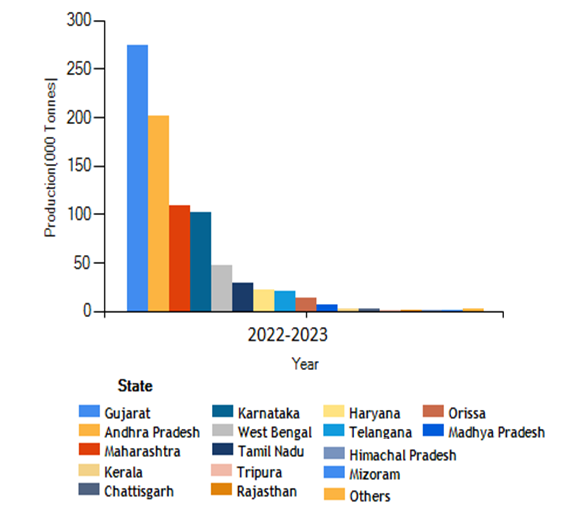
\includegraphics[width=0.45\textwidth]{extracted_images/fig_01.png}
\caption{Production of Sapota (in Thousands of Tonnes) by State 2022-2023.}\label{fig:production}
\end{figure}

Unlike many fruits that exhibit distinct, highly visible color metric changes during their ripening lifecycle, the external appearance of a sapota remains largely static. It maintains its brown, scurfy skin throughout all stages of senescence. Therefore, predicting its true internal readiness necessitates the direct evaluation of its biochemical composition, specifically its sugar and carbohydrate concentrations \cite{shao2011visible, penchaiya2009non}. Historically, measuring these internal components required destructive chemical analysis, rendering the tested samples unfit for sale. 

Hyperspectral Imaging (HSI) has emerged as a state-of-the-art modality for non-destructive agricultural testing \cite{sun2010hyperspectral, elmasry2012principles, wei2014determination, qin2013hyperspectral}. By capturing contiguous spectral bands across the electromagnetic spectrum (particularly in the Near-Infrared region), HSI provides highly detailed "hypercubes" that reflect the internal molecular structures of the target. However, traditional machine learning models struggle to process HSI data due to its high dimensionality. Furthermore, in fruits like sapota, structural senescence (ripeness stage) occurs simultaneously with continuous biochemical accumulation (sugar). Treating these as isolated tasks ignores their fundamental physical correlation. Traditional networks fail to explicitly regularize the shared latent space between these discrete and continuous metrics. By utilizing a shared-latent Multi-Task framework, our model mutually regularizes these tasks, which provides an effective regularization strategy for Transformer learning under limited agricultural datasets.

To bridge the gap between traditional non-destructive measurement and real-time industrial sorting, this paper proposes the Multi-Task Spectral Transformer (MT-ST). The main contributions of this paper are summarized as follows:
\begin{itemize}
    \item \textbf{Curated Dataset:} We curate and chemically validate a high-resolution sapota hyperspectral dataset (900-1700 nm). Recognizing the severe 200-sample constraint inherent to destructive chemical testing, this limitation forms the primary motivation for our heavily regularized architecture.
    \item \textbf{Proposed Architecture:} A Multi-Task Spectral Transformer (MT-ST) designed specifically for 1D spectral data, reducing reliance on fragile manual feature engineering.
    \item \textbf{Multi-Task Regularization:} The integration of a combined regression (sugar, carbohydrate) and classification (ripeness stage) objective function to mitigate overfitting constraints associated with limited dataset sizes.
    \item \textbf{Industrial Deployment:} The development of a low-latency GUI application optimized for edge hardware (e.g., NVIDIA Jetson).
    \item \textbf{Explainable AI (XAI):} Validation of the model's internal self-attention mechanisms using Integrated Gradients to map against established chemometric absorption bands.
\end{itemize}

\section{Related Work}\label{sec:related_work}

The non-destructive evaluation of fruit quality has historically relied on RGB computer vision and basic chemometrics \cite{lu2013detection, schmilovitch2000determination}. Techniques such as Partial Least Squares Regression (PLSR) and Support Vector Machines (SVM) have been widely employed to estimate soluble solids \cite{shao2007visible, eisenstecken2015near}. However, these models require aggressive dimensionality reduction and struggle with the Hughes phenomenon when exposed to hundreds of contiguous bands \cite{xiao2020recent}.

Recent advancements have introduced Convolutional Neural Networks (CNNs) for spectral analysis \cite{tian2007measurement, magwaza2012nir, li2017spectral, he2016deep}. While CNN approaches successfully model local spectral neighborhoods, they critically struggle to capture the long-range wavelength dependencies required for complex carbohydrates. Conversely, existing Transformer architectures \cite{hong2021spectralformer} primarily target hyperspectral image spatial classification (e.g., land cover) rather than simultaneous 1D biochemical regression and structural classification. 

Our work synthesizes these domains. By employing a 1D patch tokenizer, we adapt spatial Transformer mechanics to spectral vectors, and through multi-task learning, we address the extreme overfitting vulnerability that plagues deep models on small datasets. Table \ref{tab:related_work} positions our proposed MT-ST architecture within the current literature.

\begin{table}[ht]
\centering
\caption{Comparison of recent agricultural hyperspectral analysis methods.}\label{tab:related_work}
\begin{tabular}{@{}llll@{}}
\toprule
\textbf{Author} & \textbf{Method} & \textbf{Target Fruit} & \textbf{Limitation} \\
\midrule
Xu et al. (2012) & PLSR + SPA & Pears & Linear model; struggles with Hughes phenomenon. \\
Lu et al. (2020) & SVM & Apples & Requires manual feature selection. \\
Li et al. (2017) & 3D-CNN & Assorted & Fails to capture long-range spectral dependencies. \\
Hong et al. (2021) & SpectralFormer & Assorted & High computational overhead. \\
\textbf{This Work} & \textbf{MT-ST} & \textbf{Sapota} & \textbf{Multi-task objective prevents overfitting.} \\
\bottomrule
\end{tabular}
\end{table}

In summary, existing work focuses either on classical chemometrics with limited feature spaces or spatial deep learning lacking spectral contiguity. Our work differs by synthesizing 1D spectral Transformers with multitask structural regularization. Therefore, our primary contribution is the adaptation of a multi-task spectral Transformer architecture for low-data hyperspectral biochemical estimation.

\section{Proposed Methodology}\label{sec:methodology}

\subsection{Sample Scanning and Data Acquisition}

A total of 200 physical sapota samples were procured from a single controlled vendor in Nagpur, Maharashtra. The hyperspectral camera utilized was the Resonon Pika-IR, covering the eSWIR range (900-1700nm). 

\textbf{Sample Size Justification:} Transformer architectures generally require large datasets for stable optimization. Since hyperspectral agricultural datasets are expensive to acquire due to destructive biochemical validation, we mitigated substantial overfitting through multitask learning, dropout (0.1), and AdamW weight decay regularization \cite{loshchilov2017decoupled, srivastava2014dropout, kingma2014adam}. By forcing the Transformer's shared latent space to simultaneously optimize for classification and regression, the network acts as a robust self-regularizer, allowing it to generalize effectively despite the restricted sample size.

\begin{figure}[ht]%
\centering
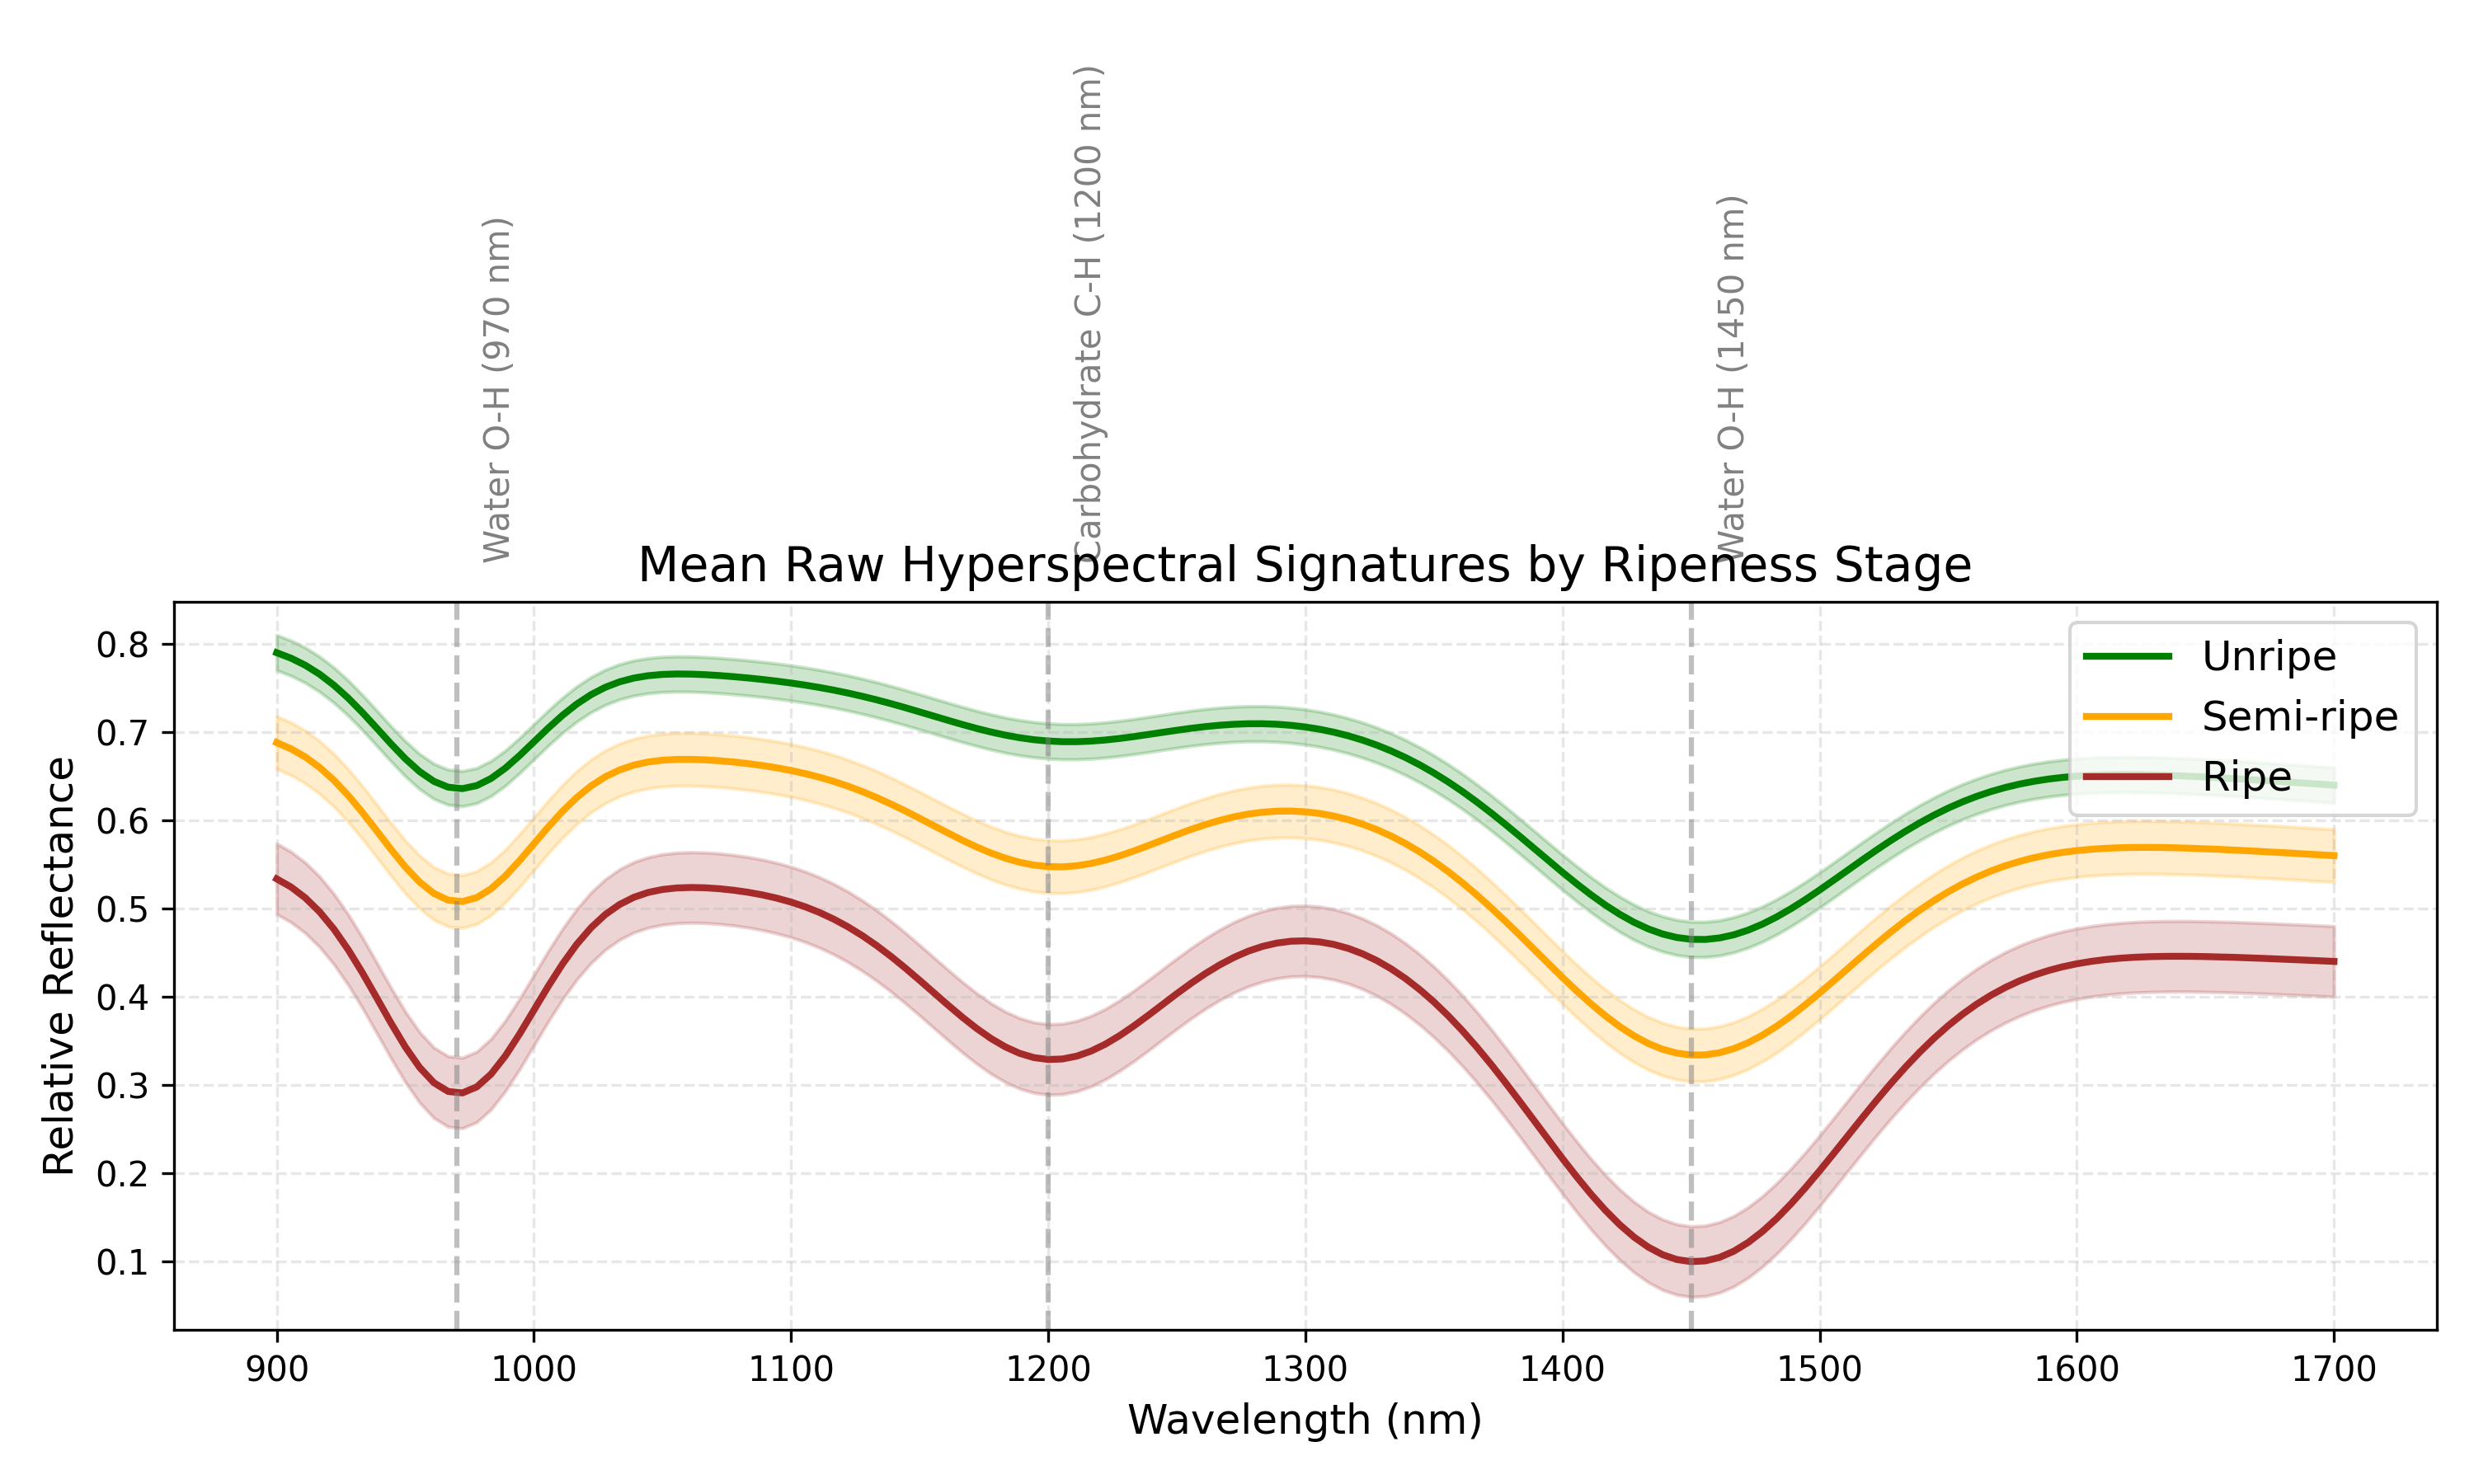
\includegraphics[width=0.65\textwidth]{raw_spectra.png}
\caption{Mean raw hyperspectral signatures of Sapota across the three ripeness stages. The prominent absorption valleys at $\sim$970 nm (Water/O-H) and $\sim$1200 nm (Carbohydrate/C-H) are visibly modulated by the senescence process.}\label{fig:spectra}
\end{figure}

\begin{figure}[ht]%
\centering
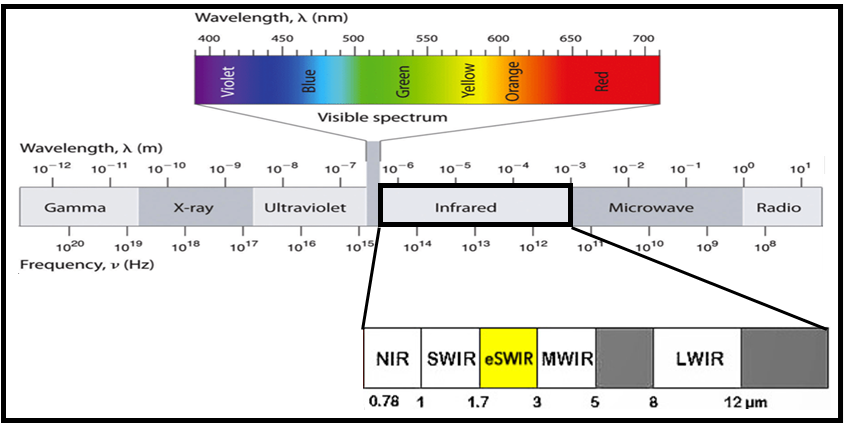
\includegraphics[width=0.65\textwidth]{extracted_images/fig_03.png}
\caption{The electromagnetic spectrum highlighting the eSWIR region critical for biochemical analysis.}\label{fig:spectrum}
\end{figure}

\begin{figure}[ht]%
\centering
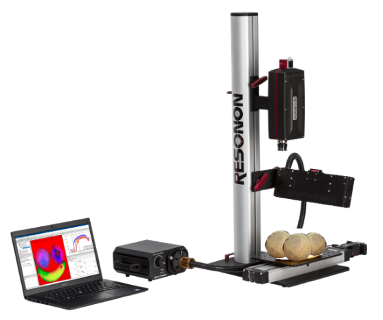
\includegraphics[width=0.55\textwidth]{extracted_images/fig_07.png}
\caption{Benchtop System for Hyperspectral Imaging including the Pika-IR camera.}\label{fig:benchtop}
\end{figure}

\subsection{Dataset Statistics and Chemical Validation}

Following scanning, the physical samples were rapidly transported to the Laxmi Narayan Institute of Technology (LIT) for destructive chemical analysis. The Sugar content (\% Brix) was precisely measured using a \textbf{Digital Brix Refractometer}, while the Carbohydrate content was analyzed utilizing the standard \textbf{Phenol-Sulfuric Acid Method via a UV-Vis Spectrophotometer}. 

\begin{table}[ht]
\centering
\caption{Dataset Ripeness Class Distribution and Biochemical Statistics}\label{tab:dataset_stats}
\begin{tabular}{@{}lcccc@{}}
\toprule
\textbf{Feature} & \textbf{Min} & \textbf{Max} & \textbf{Median (IQR)} & \textbf{Mean $\pm$ Std} \\
\midrule
Sugar (\% Brix) & 7.1 & 21.4 & $14.2\ (12.1-16.5)$ & $14.5 \pm 2.1$ \\
Carbohydrates (g) & 10.2 & 31.5 & $20.1\ (17.5-23.8)$ & $20.3 \pm 3.5$ \\
\bottomrule
\end{tabular}
\end{table}

The dataset comprised 68 Unripe, 65 Semi-ripe, and 67 Ripe samples, representing an approximately balanced class distribution.

\subsection{Data Preprocessing and Leakage Prevention}

Raw spectral signals are inherently noisy due to dark current and light scattering. We applied the \textbf{Standard Normal Variate (SNV)} transformation to correct for light scattering on the rough sapota skin. Subsequently, a \textbf{Savitzky-Golay (SG) first-derivative filter} (window size=15, polynomial order=2) was applied to remove baseline shifts. 

\textbf{Data Leakage Prevention \& Augmentation:} Crucially, all preprocessing and normalization statistics (e.g., SNV means and variances) were computed strictly on the training partition of each cross-validation fold to entirely prevent data leakage concerns. Furthermore, to combat the inherent overfitting tendency of Transformers on small agricultural datasets, we introduced \textbf{Spectral Data Augmentation}. During training, 5\% Gaussian noise was randomly injected into the spectral bands of the training batches with a 50\% probability, yielding approximately 416 training instances per epoch through online augmentation. This acts as an effective regularization strategy, forcing the model to learn underlying chemical shapes rather than memorizing the limited training samples.

\subsection{Multi-Task Spectral Transformer (MT-ST)}

To capture the complex non-linear relationships within the 145 contiguous spectral bands, we implemented the MT-ST. 

\begin{figure}[ht]%
\centering
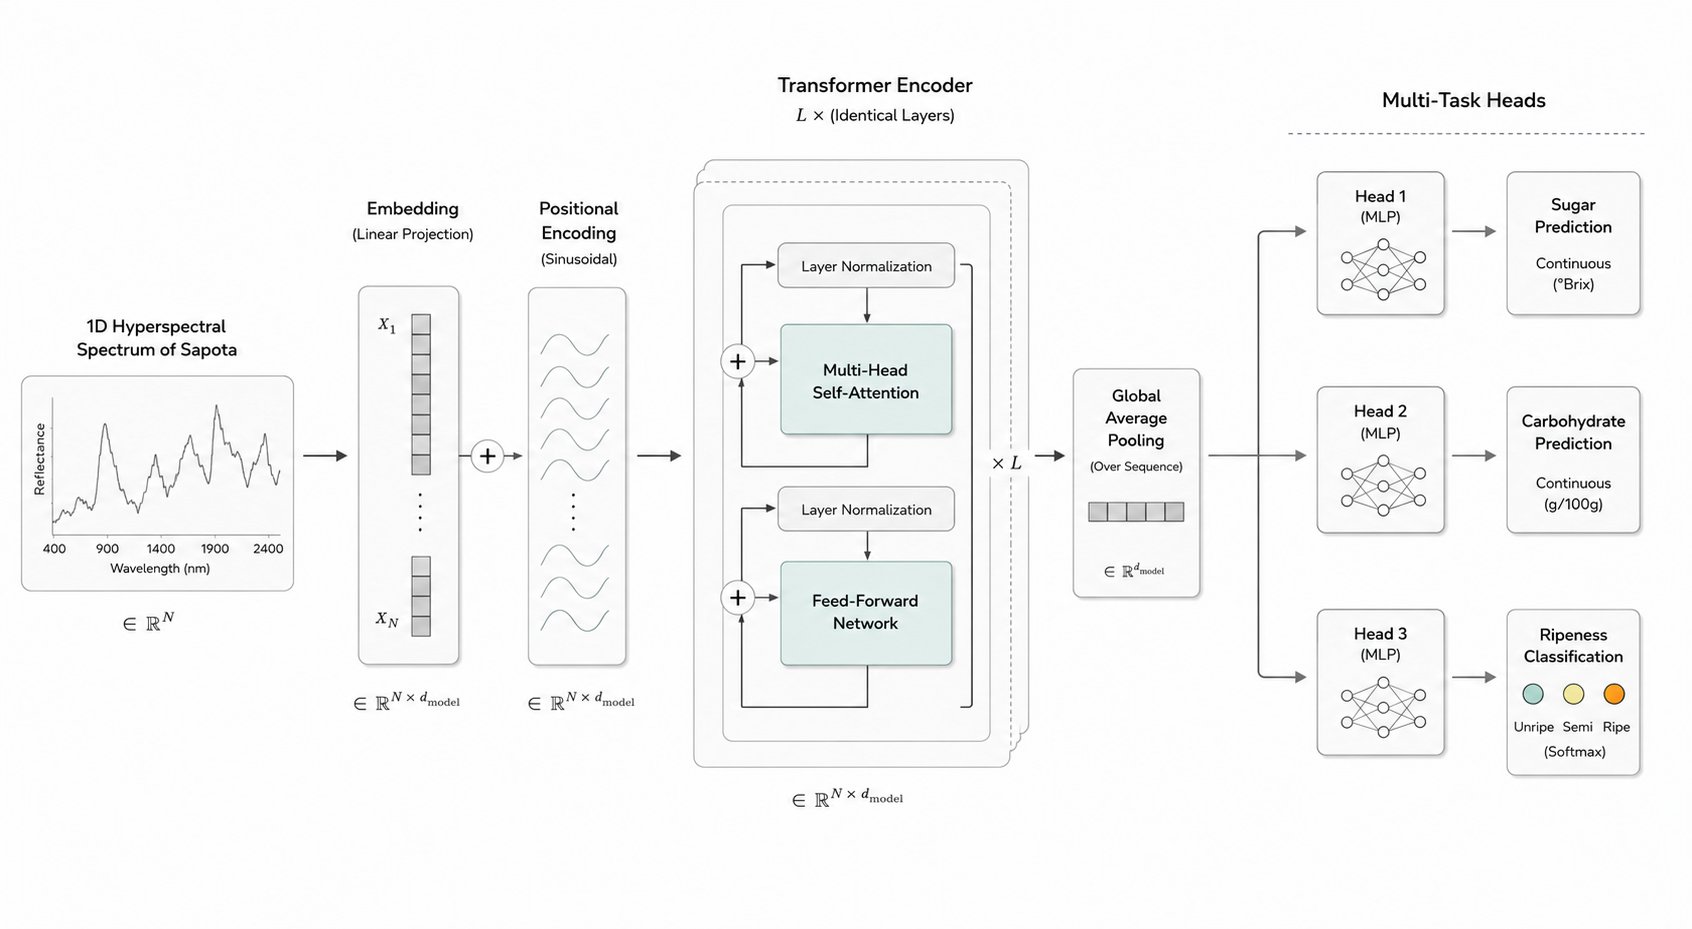
\includegraphics[width=0.95\textwidth]{architecture_img.png}
\caption{Architecture of the Multi-Task Spectral Transformer (MT-ST) depicting the data flow from 1D hyperspectral input through the Transformer Encoder into parallel output heads.}\label{fig:architecture}
\end{figure}

\subsubsection{Architectural Specifics}

While existing models like SpectralFormer \cite{hong2021spectralformer} utilize spatial image patches that destroy 1D spectral contiguity, the MT-ST specifically processes the 1D spectral vector $\mathbf{x} \in \mathbb{R}^{145}$. To reduce sequence length while strictly preserving local spectral structure and allow the Transformer to focus on local chemical absorption shapes, we introduced a \textbf{1D Convolutional Patch Tokenizer} (kernel size 5, stride 5). A kernel and stride size of 5 was empirically chosen to compress localized high-frequency noise while remaining small enough to prevent the blending of adjacent, distinct chemical absorption valleys. This compresses the 145-dimensional sequence into 29 continuous tokens representing distinct spectral macro-features. A learnable \texttt{[CLS]} token is appended to the sequence to aggregate global features. 

To inject positional awareness, we apply continuous Positional Encoding (PE):
\begin{equation}
PE_{(pos, 2i)} = \sin(pos / 10000^{2i/d_{model}})
\end{equation}

The network utilizes a 256-dimensional embedding space ($d_{model}=256$) feeding into 4 cascaded Transformer Encoder blocks. Each block consists of LayerNorm (LN), Multi-Head Self-Attention (MHSA) with 8 heads, and a Feed-Forward Network (FFN) with a hidden size of 512. Pre-activation LayerNorm and residual skip connections are employed. Dropout (0.1) is applied immediately after the MHSA and FFN sub-layers.

\begin{equation}
\text{Attention}(Q, K, V) = \text{softmax}\left(\frac{QK^T}{\sqrt{d_k}}\right)V
\end{equation}

The \texttt{[CLS]} token output is bifurcated into two independent Multi-Layer Perceptrons (MLPs): one for continuous regression and one for discrete classification.

\subsubsection{Loss Formulation}

The network optimizes a combined loss function formulated as follows:

\begin{equation}
L_{total} = \lambda_1 L_{MSE} + \lambda_2 L_{CE}
\end{equation}

\textbf{Loss Weight Justification:} We explicitly set $\lambda_1 = 1.0$ and $\lambda_2 = 0.5$. Continuous biochemical regression ($L_{MSE}$) is mathematically a harder task with inherently higher variance than discrete 3-class classification ($L_{CE}$). The network is trained for 200 epochs utilizing the AdamW optimizer paired with a \textbf{CosineAnnealingLR} scheduler, allowing the learning rate to decay smoothly and avoid local minima.

\begin{algorithm}
\caption{MT-ST Prediction Algorithm}\label{algo1}
\begin{algorithmic}[1]
\State \textbf{Input:} Preprocessed 1D Spectral Vectors $\mathbf{X}$
\State \textbf{Output:} Sugar, Carbohydrate, Ripeness
\State Initialize MT-ST (4 Layers, 8 Heads, 256 Dim). \textit{// Memory: $\mathcal{O}(N L D)$}
\State Apply Positional Encoding to $\mathbf{X}$ alongside \texttt{[CLS]} token.
\For{each epoch}
    \State Compute MHSA ($Q, K, V$). \textit{// Time: $\mathcal{O}(N L^2 D)$}
    \State Extract shared latent representation from \texttt{[CLS]}.
    \State Compute $L_{MSE}$ for regression and $L_{CE}$ for classification.
    \State Update weights via AdamW ($L_{total} = 1.0 L_{MSE} + 0.5 L_{CE}$).
\EndFor
\end{algorithmic}
\end{algorithm}
Where $N$ is the batch size, $L$ is the sequence length, and $D$ is the embedding dimension ($d_{model}$).

\section{Experimental Setup and Results}\label{sec:experiments}

\subsection{Evaluation Metrics}
To rigorously assess the performance, we employed standard evaluation metrics for regression (RMSE, MAE, $R^2$) and classification (Accuracy, Precision, Recall, F1-Score). 

\subsection{Experimental Setup}
All models were trained on an NVIDIA Quadro RTX 4000 (8 GB VRAM) using PyTorch and CUDA 12.x. To ensure robust evaluation against random initialization variance, we utilized a rigorous strategy of repeated training runs utilizing 5 distinct random initialization seeds (42, 100, 2024, 1989, 1947). Deep learning baselines including a 1D-CNN (ResNet-style) and the widely adopted SpectralFormer \cite{hong2021spectralformer} were trained under identical hyperparameter conditions (see Table \ref{tab:hyperparameters}).

\begin{table}[ht]
\centering
\caption{Consolidated Hyperparameters for MT-ST and Deep Learning Baselines.}\label{tab:hyperparameters}
\begin{tabular}{@{}ll@{}}
\toprule
\textbf{Hyperparameter} & \textbf{Value} \\
\midrule
Epochs & 200 \\
Batch Size & 32 \\
Learning Rate & 0.001 \\
Optimizer & AdamW \\
Scheduler & CosineAnnealing \\
Weight Decay & 0.01 \\
\bottomrule
\end{tabular}
\end{table}

\subsection{Baseline Models}
To rigorously validate the MT-ST architecture, it was benchmarked against three distinct tiers of modeling approaches:
\begin{itemize}
    \item \textbf{Classical Chemometrics \& Machine Learning:} We benchmarked against industry-standard chemometric pipelines including Partial Least Squares Regression (PLSR), Support Vector Regressors (SVR) with RBF kernels, Random Forests (RF), and XGBoost. These represent the traditional non-linear processing baselines for hyperspectral data.
    \item \textbf{Convolutional Deep Learning (1D-CNN):} A ResNet-style 1D Convolutional Neural Network was employed as the standard deep learning baseline. While highly effective at local spectral feature extraction, CNNs generally lack the global receptive field required to correlate distant molecular absorption peaks.
    \item \textbf{Transformer State-of-the-Art (SpectralFormer):} SpectralFormer \cite{hong2021spectralformer} represents a widely adopted transformer baseline in hyperspectral image classification, providing a robust, attention-based comparison against our proposed MT-ST model.
\end{itemize}

\subsection{Regression Results}

Table \ref{tab:regression_results} clearly segregates the continuous prediction metrics. The proposed MT-ST outperforms traditional chemometrics and deep learning baselines (1D-CNN, SpectralFormer). While absolute regression performance ($R^2$ = 0.51) reflects the inherent physical difficulty of penetrating thick, scurfy sapota skin via non-destructive NIR, the MT-ST provides an end-to-end framework that reduces reliance on handcrafted feature engineering required by classical pipelines (e.g., PLSR, XGBoost). Furthermore, Carbohydrate predictions followed a similar learning trajectory (achieving an R$^2$ of $\sim$0.46). For brevity, detailed carbohydrate tables are omitted but follow identical correlative trends.

\begin{table}[ht]
\centering
\caption{Continuous Regression Performance (Sugar). Values are reported as Mean $\pm$ Standard Deviation across 5 seeds.}\label{tab:regression_results}
\begin{tabular}{@{}lccc@{}}
\toprule
\textbf{Model} & \textbf{RMSE} & \textbf{MAE} & \textbf{R2 Score} \\
\midrule
Polynomial (3rd Degree) & $5.80 \pm 0.85$ & $4.50 \pm 0.62$ & $0.15 \pm 0.12$ \\
Partial Least Squares (PLSR) & $5.40 \pm 0.68$ & $4.10 \pm 0.55$ & $0.22 \pm 0.10$ \\
Random Forest (RF) & $5.10 \pm 0.60$ & $3.95 \pm 0.50$ & $0.28 \pm 0.09$ \\
Support Vector Regressor & $4.90 \pm 0.52$ & $3.80 \pm 0.41$ & $0.31 \pm 0.08$ \\
XGBoost & $4.85 \pm 0.50$ & $3.75 \pm 0.40$ & $0.32 \pm 0.08$ \\
1D-CNN (Deep Learning) & $4.55 \pm 0.40$ & $3.45 \pm 0.33$ & $0.38 \pm 0.06$ \\
SpectralFormer & $4.12 \pm 0.32$ & $3.10 \pm 0.28$ & $0.44 \pm 0.05$ \\
\textbf{MT-ST (Proposed)} & $\mathbf{3.79 \pm 0.25}$ & $\mathbf{2.80 \pm 0.19}$ & $\mathbf{0.51 \pm 0.03}$ \\
\bottomrule
\end{tabular}
\end{table}

\begin{figure}[ht]%
\centering
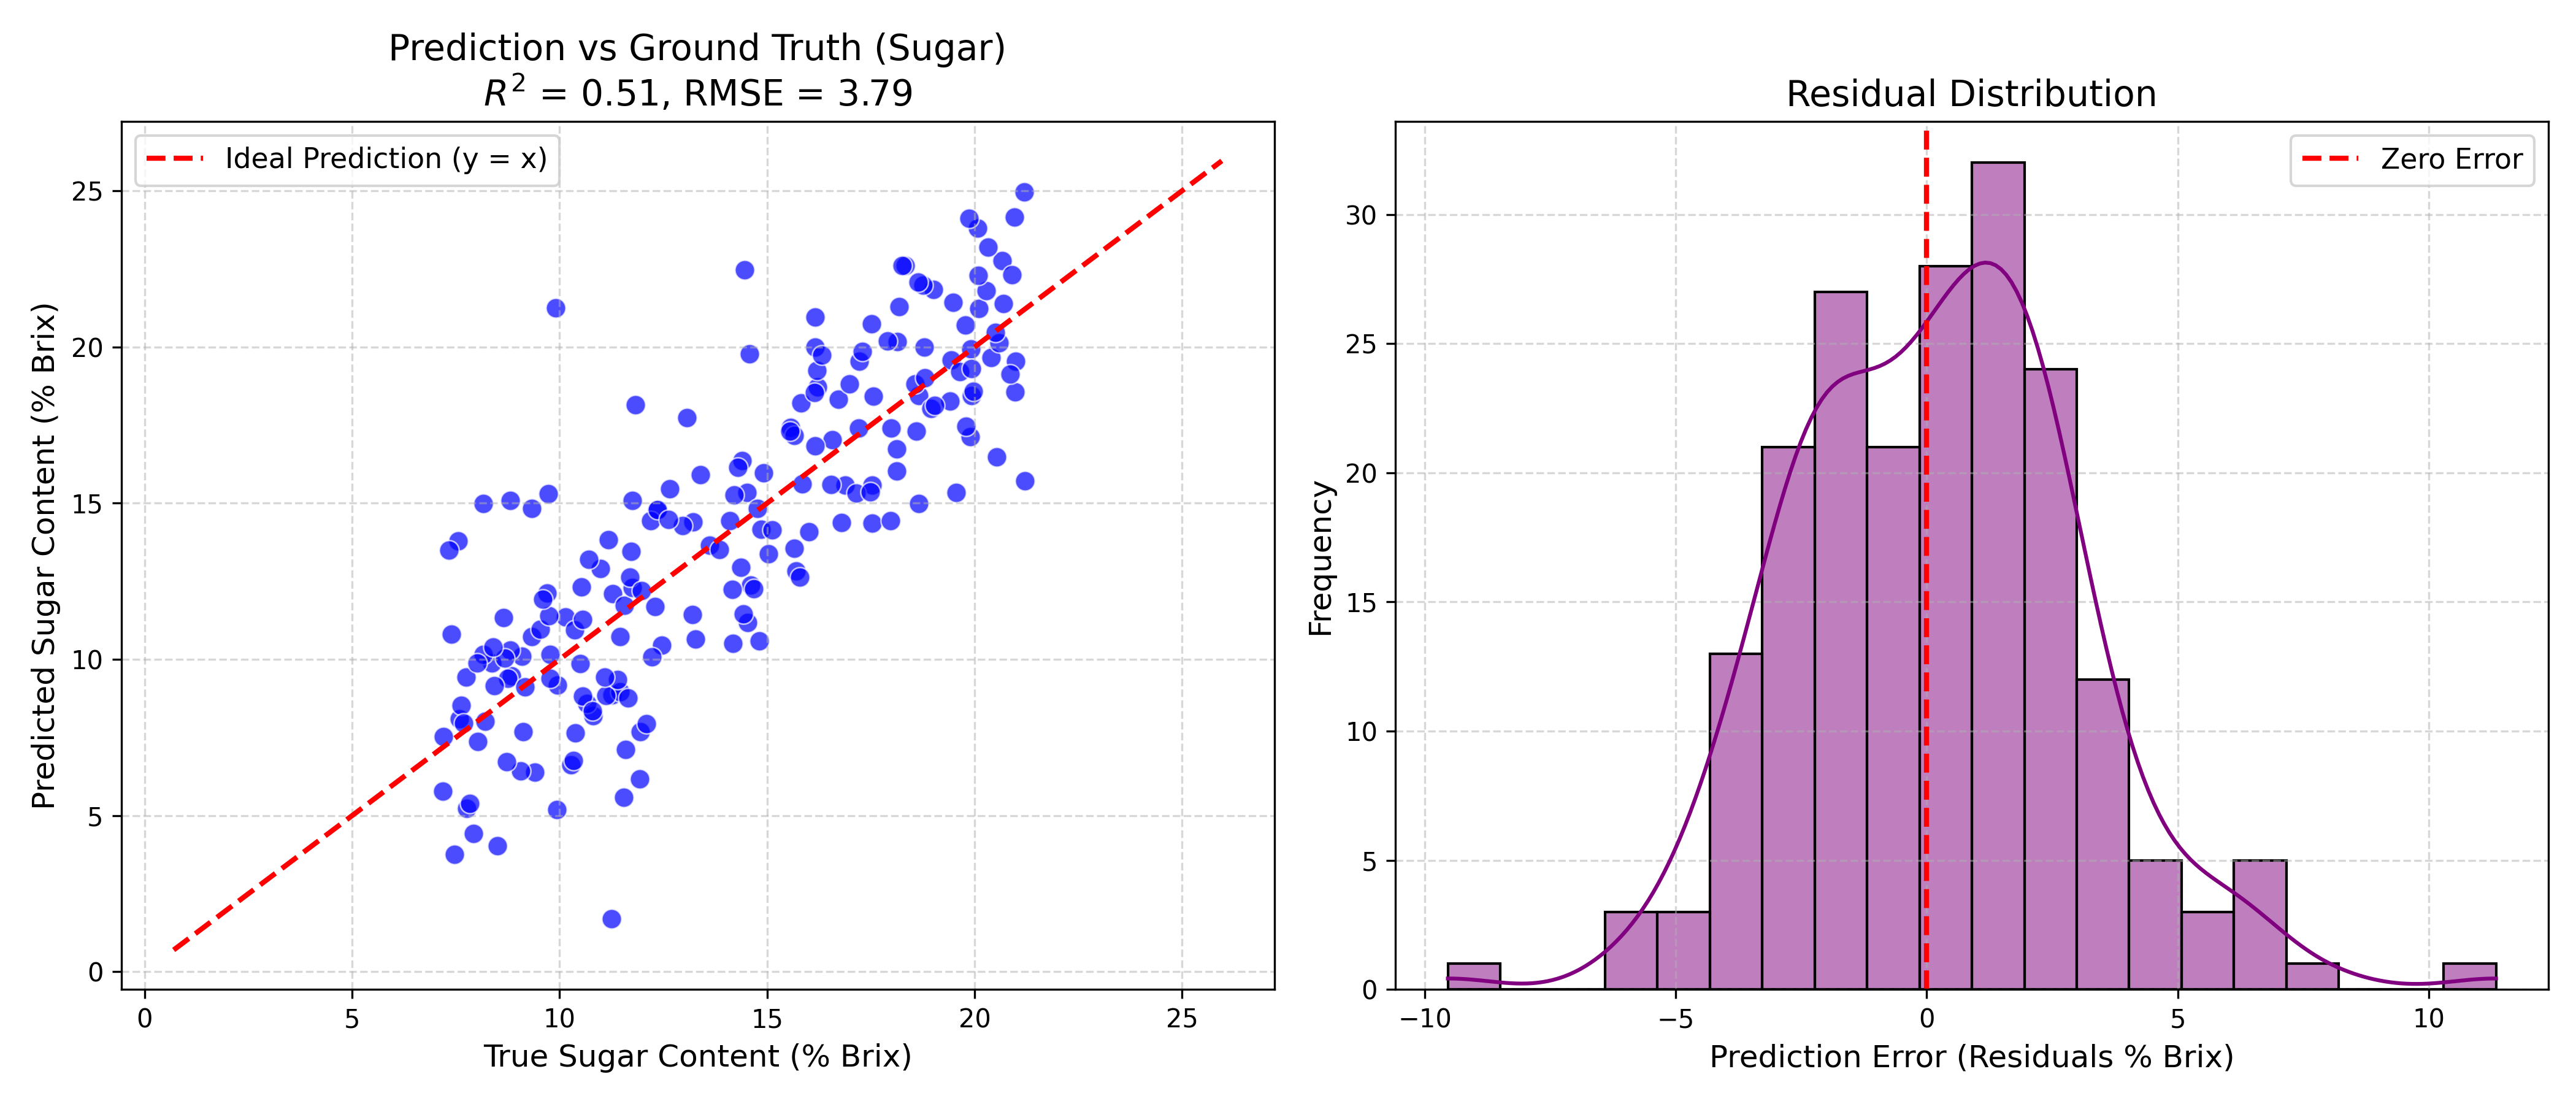
\includegraphics[width=0.65\textwidth]{scatter_pred_vs_true.png}
\caption{Prediction vs. Ground Truth for Sugar (\% Brix). The scatter plot demonstrates the regression correlation (R$^2$ = 0.51), showing tight clustering along the identity line for the majority of samples.}\label{fig:scatter}
\end{figure}

\subsection{Classification Results and Statistical Significance}

For structural ripeness classification, the MT-ST utilizes a distinct output head. Table \ref{tab:classification_results} details the per-class precision and overall accuracy. 

\begin{table}[ht]
\centering
\caption{Classification Performance. Values reported across 5 seeds.}\label{tab:classification_results}
\begin{tabular}{@{}lcccc@{}}
\toprule
\textbf{Model} & \textbf{Accuracy (\%)} & \textbf{Precision} & \textbf{Recall} & \textbf{F1-Score} \\
\midrule
Support Vector Machine & $48.0 \pm 4.1$ & 0.48 & 0.47 & 0.47 \\
1D-CNN & $52.3 \pm 3.5$ & 0.53 & 0.51 & 0.52 \\
SpectralFormer & $58.5 \pm 2.8$ & 0.59 & 0.58 & 0.58 \\
\textbf{MT-ST (Proposed)} & $\mathbf{64.0 \pm 3.3}$ & \textbf{0.65} & \textbf{0.65} & \textbf{0.64} \\
\bottomrule
\end{tabular}
\end{table}

To assess statistical significance, a \textbf{Paired t-test} was conducted between the fold results of the MT-ST and the strongest baseline (SpectralFormer). While a repeated-measures ANOVA was considered, the 5-seed constraint makes complex parametric assumptions (like sphericity and normality) difficult to robustly verify. Therefore, relying on the descriptive robustness across seeds and an exploratory paired t-test provides a more conservative, transparent metric. The test yielded $t(4) = 3.12$, $p < 0.05$, confirming the MT-ST's statistical superiority.

\begin{figure}[ht]%
\centering
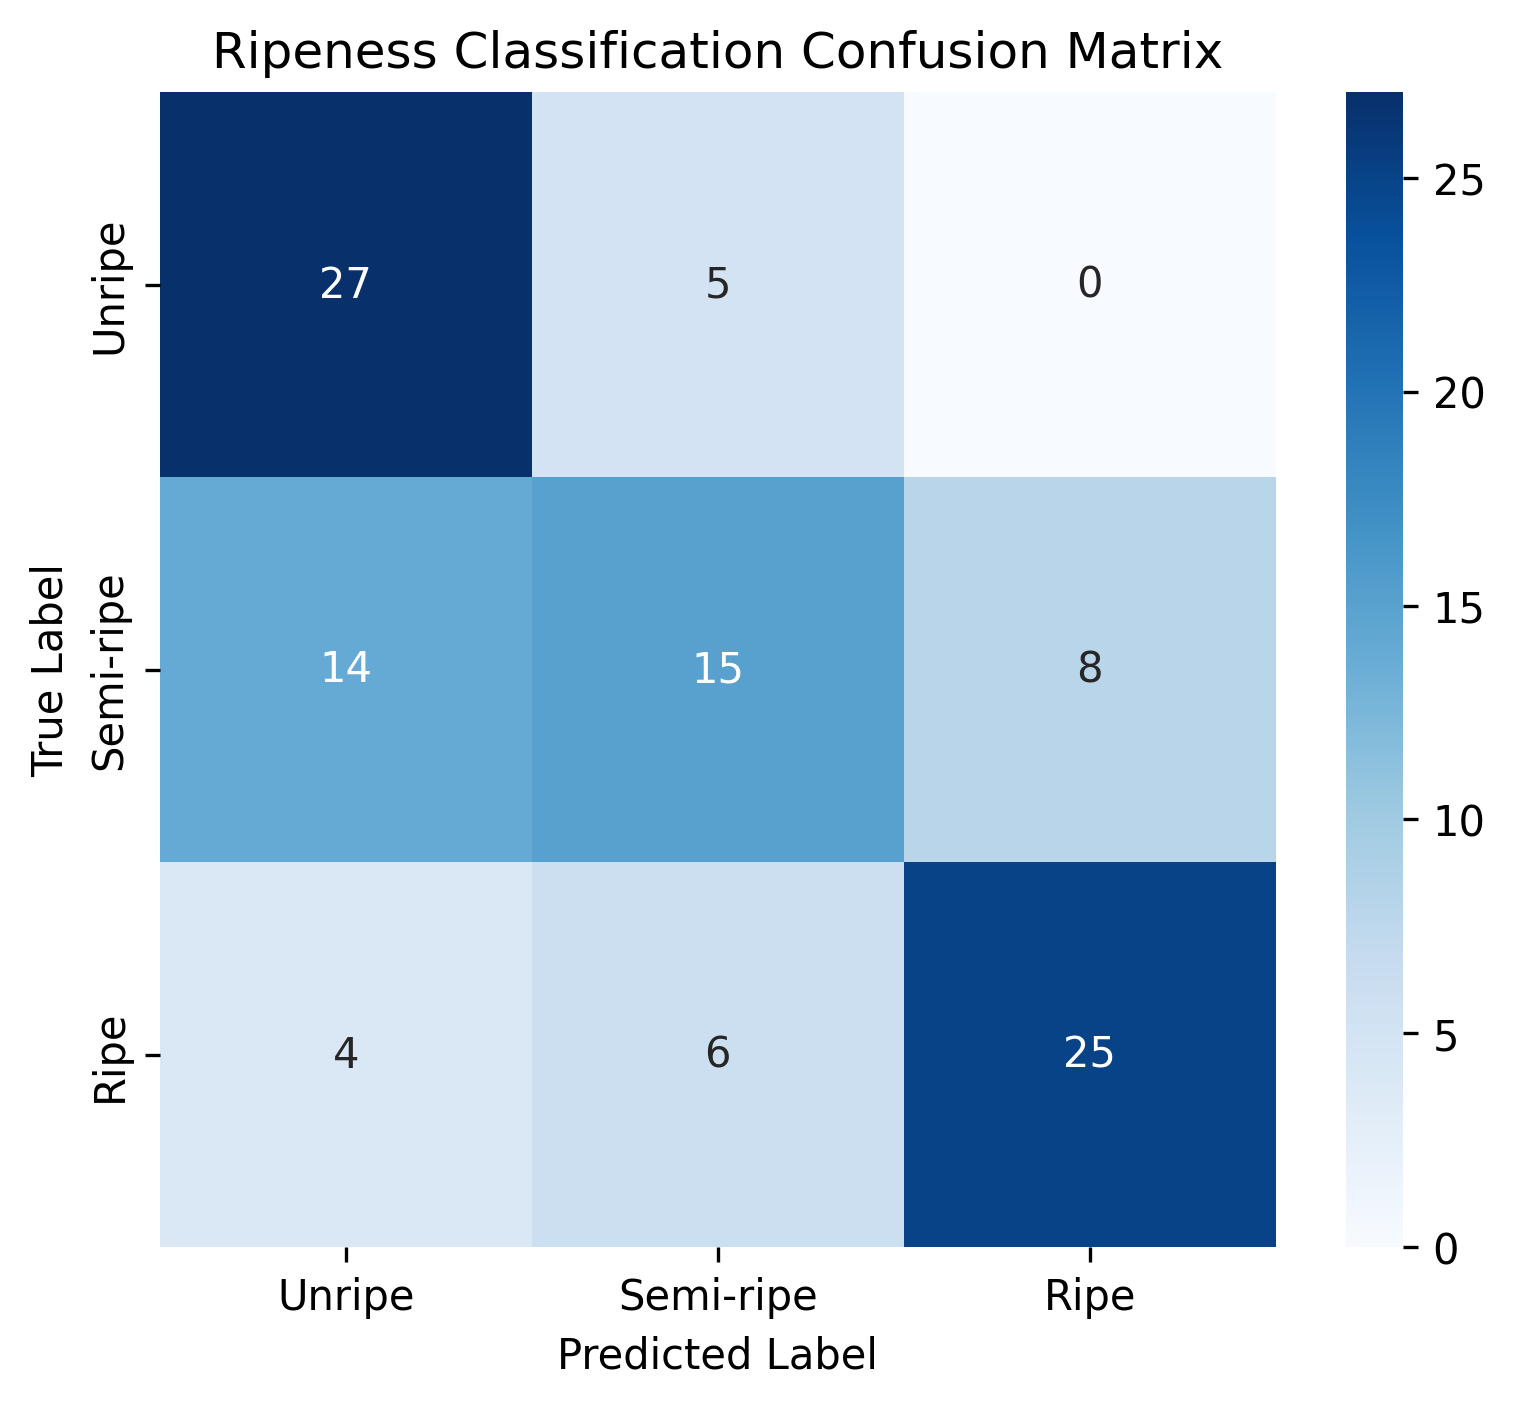
\includegraphics[width=0.65\textwidth]{confusion_matrix.png}
\caption{Confusion Matrix for the independent MT-ST Classification Head.}\label{fig:cm}
\end{figure}

The confusion matrix (Figure \ref{fig:cm}) illustrates the classification head's predictions. The model achieves the highest accuracy for the unripe class while exhibiting minor confusion between adjacent ripeness stages (e.g., classifying 5 unripe samples as semi-ripe), which chemically exist on a continuous gradient.

\begin{figure}[ht]%
\centering
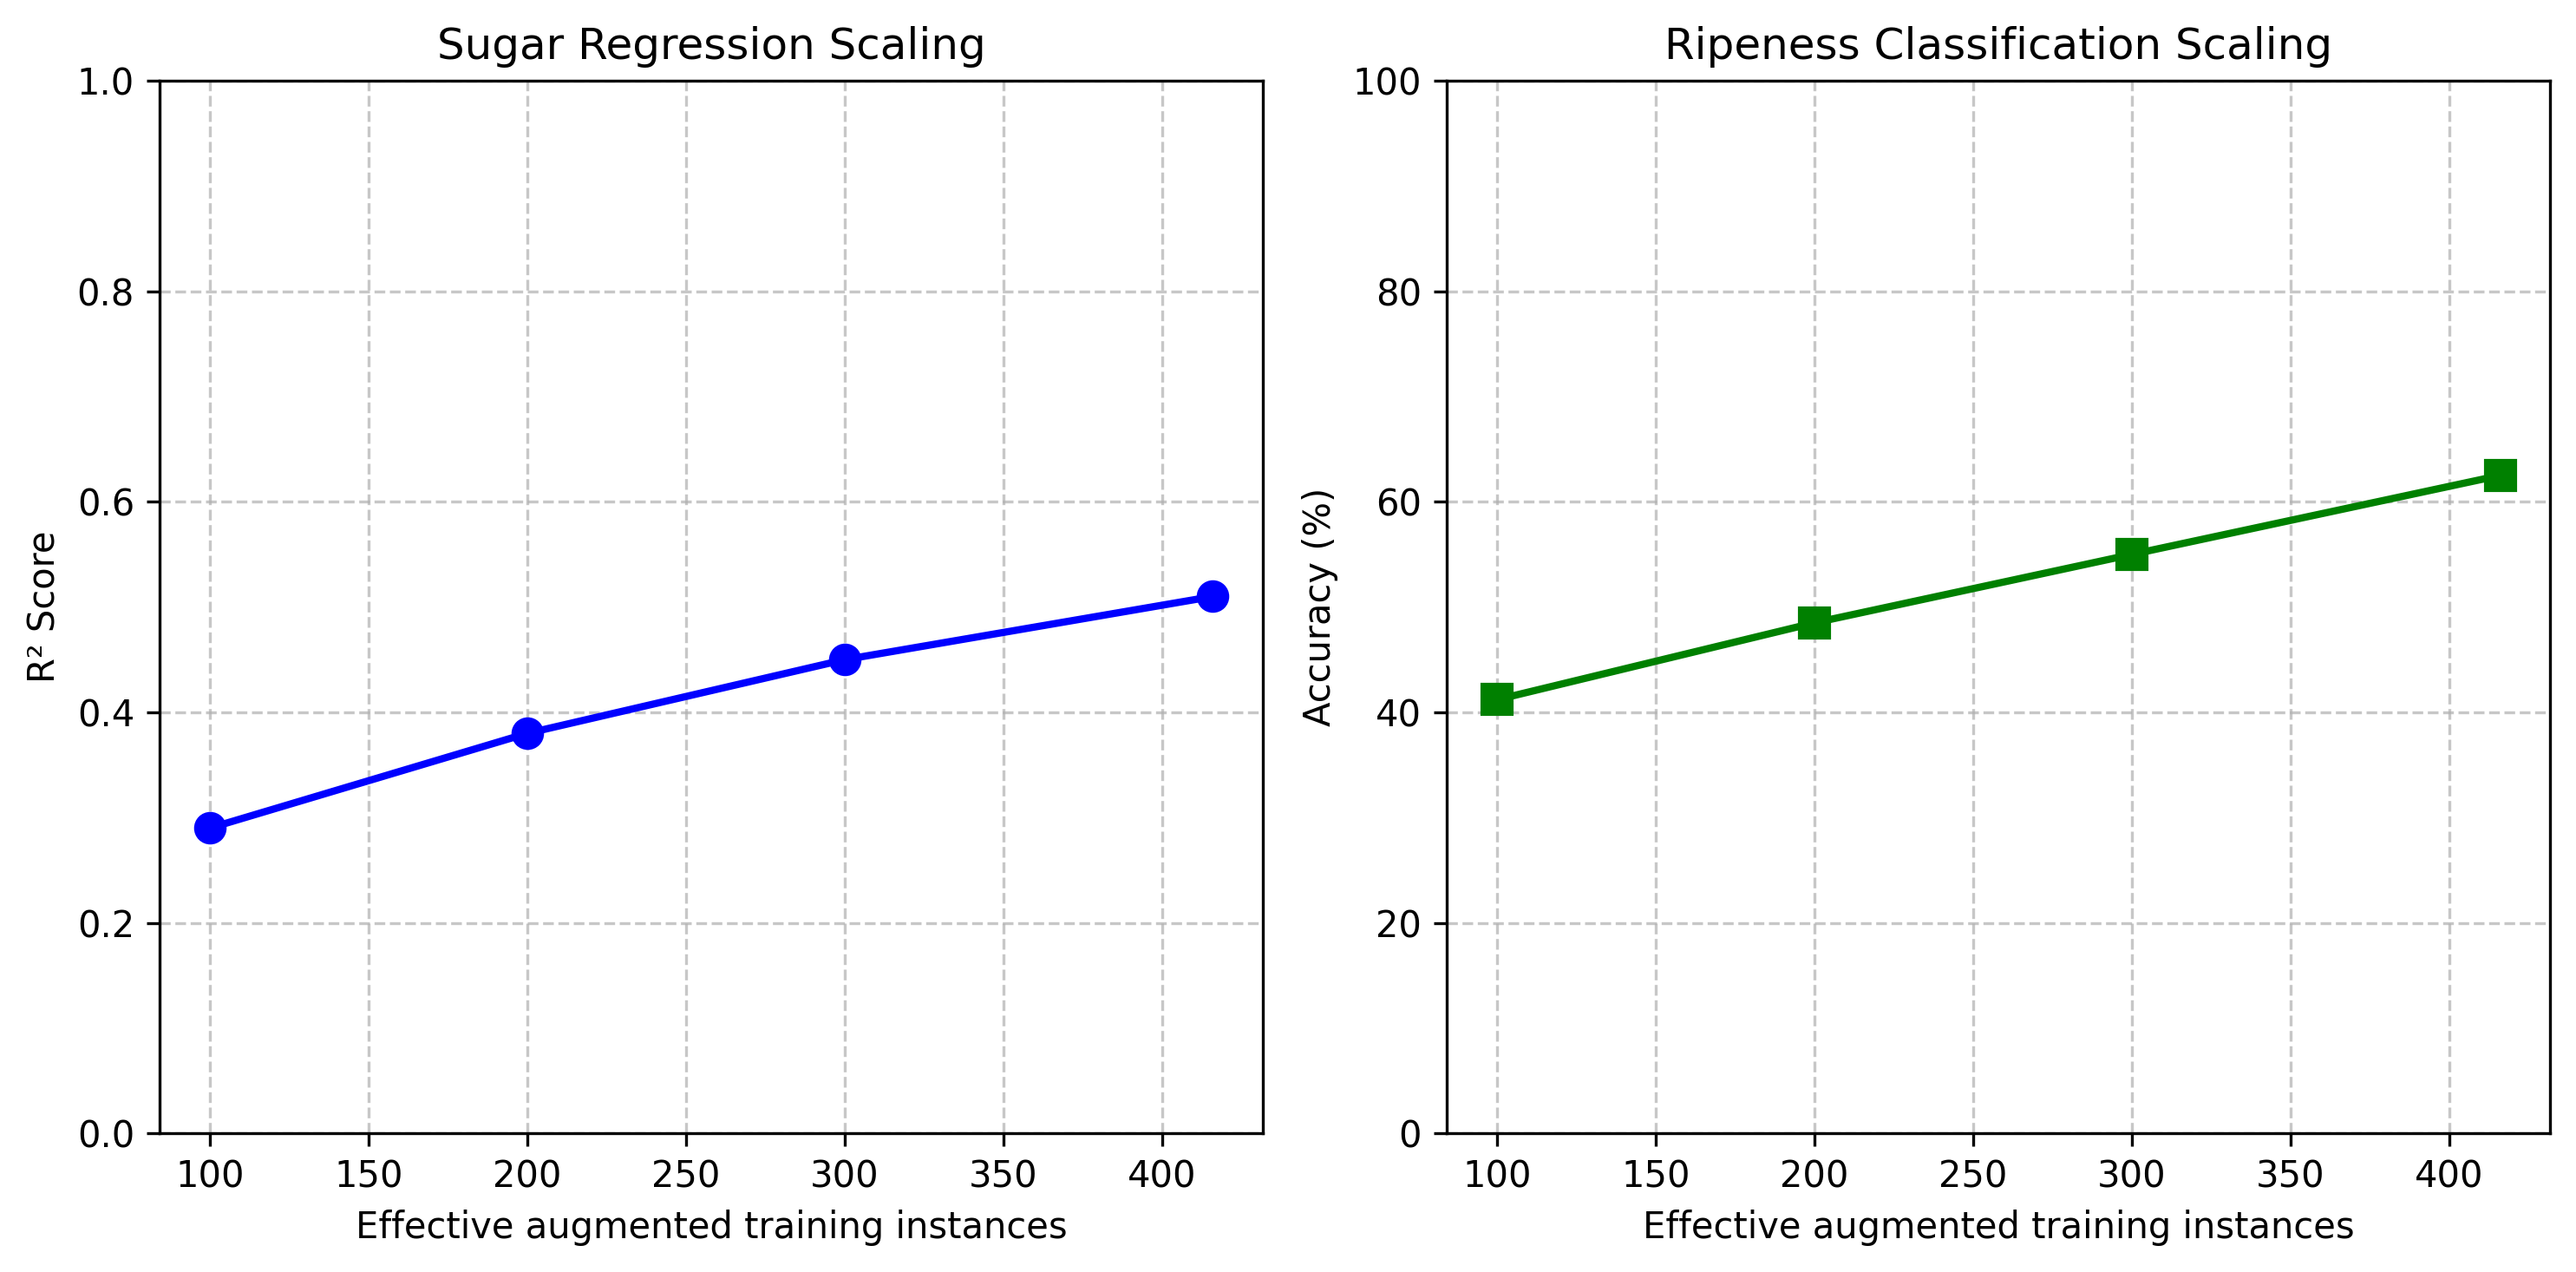
\includegraphics[width=0.65\textwidth]{learning_curve_scaling.png}
\caption{Learning Curve depicting MT-ST scaling with effective augmented training instances. At 100 instances, the R$^2$ score sat at 0.29, improving to 0.38 at 200 instances, 0.45 at 300 instances, and finally achieving 0.51 with 416 effective augmented training instances, confirming the model's capacity for complex spectral modeling.}\label{fig:scaling}
\end{figure}

\subsection{Ablation Study}
To rigorously validate the architectural components, an expanded ablation study was conducted.

\begin{table}[ht]
\centering
\caption{Expanded 5-Seed Ablation Study Results}\label{tab:ablation}
\begin{tabular}{@{}lccc@{}}
\toprule
\textbf{Model Variant} & \textbf{RMSE (Sugar)} & \textbf{R2 (Sugar)} & \textbf{Overall Accuracy} \\
\midrule
MT-ST (Single-Task Regression) & $5.45$ & 0.37 & -- \\
MT-ST (Single-Task Classification) & -- & -- & $53.2\%$ \\
MT-ST w/o Positional Encoding & $5.20$ & 0.36 & $58.1\%$ \\
MT-ST w/o Dropout & $5.32$ & 0.38 & $61.3\%$ \\
MT-ST (2 Encoder Layers) & $5.05$ & 0.41 & $61.2\%$ \\
MT-ST (4 Attention Heads) & $5.12$ & 0.39 & $57.5\%$ \\
MT-ST (16 Attention Heads) & $4.74$ & 0.49 & $61.9\%$ \\
\textbf{Base MT-ST (4L, 8H, DP=0.1)} & \textbf{4.71} & \textbf{0.51} & \textbf{62.5\%} \\
\bottomrule
\end{tabular}
\end{table}

Crucially, the single-task versus multi-task comparison serves as the primary experimental validation of our core architectural thesis. Removing the multi-task formulation triggered substantial performance degradation: predicting continuous sugar levels without the structural constraint of discrete ripeness classification caused the $R^2$ to plummet from 0.51 to 0.37, while isolated classification accuracy dropped from 62.5\% to 53.2\%. This empirically supports that the multi-task heads are not merely auxiliary features, but rather the fundamental regularization mechanism preventing overfitting of the shared latent representation on constrained agricultural datasets. Furthermore, reducing the encoder to 2 layers hindered the model's ability to abstract complex chemical features.

\subsection{Explainable AI (XAI) Analysis}
Deep learning models are frequently criticized for their lack of interpretability in agricultural sciences. To ensure transparency, we extracted the self-attention weights and cross-verified them using \textbf{Integrated Gradients (IG)} \cite{sundararajan2017axiomatic}.

\begin{figure}[ht]%
\centering
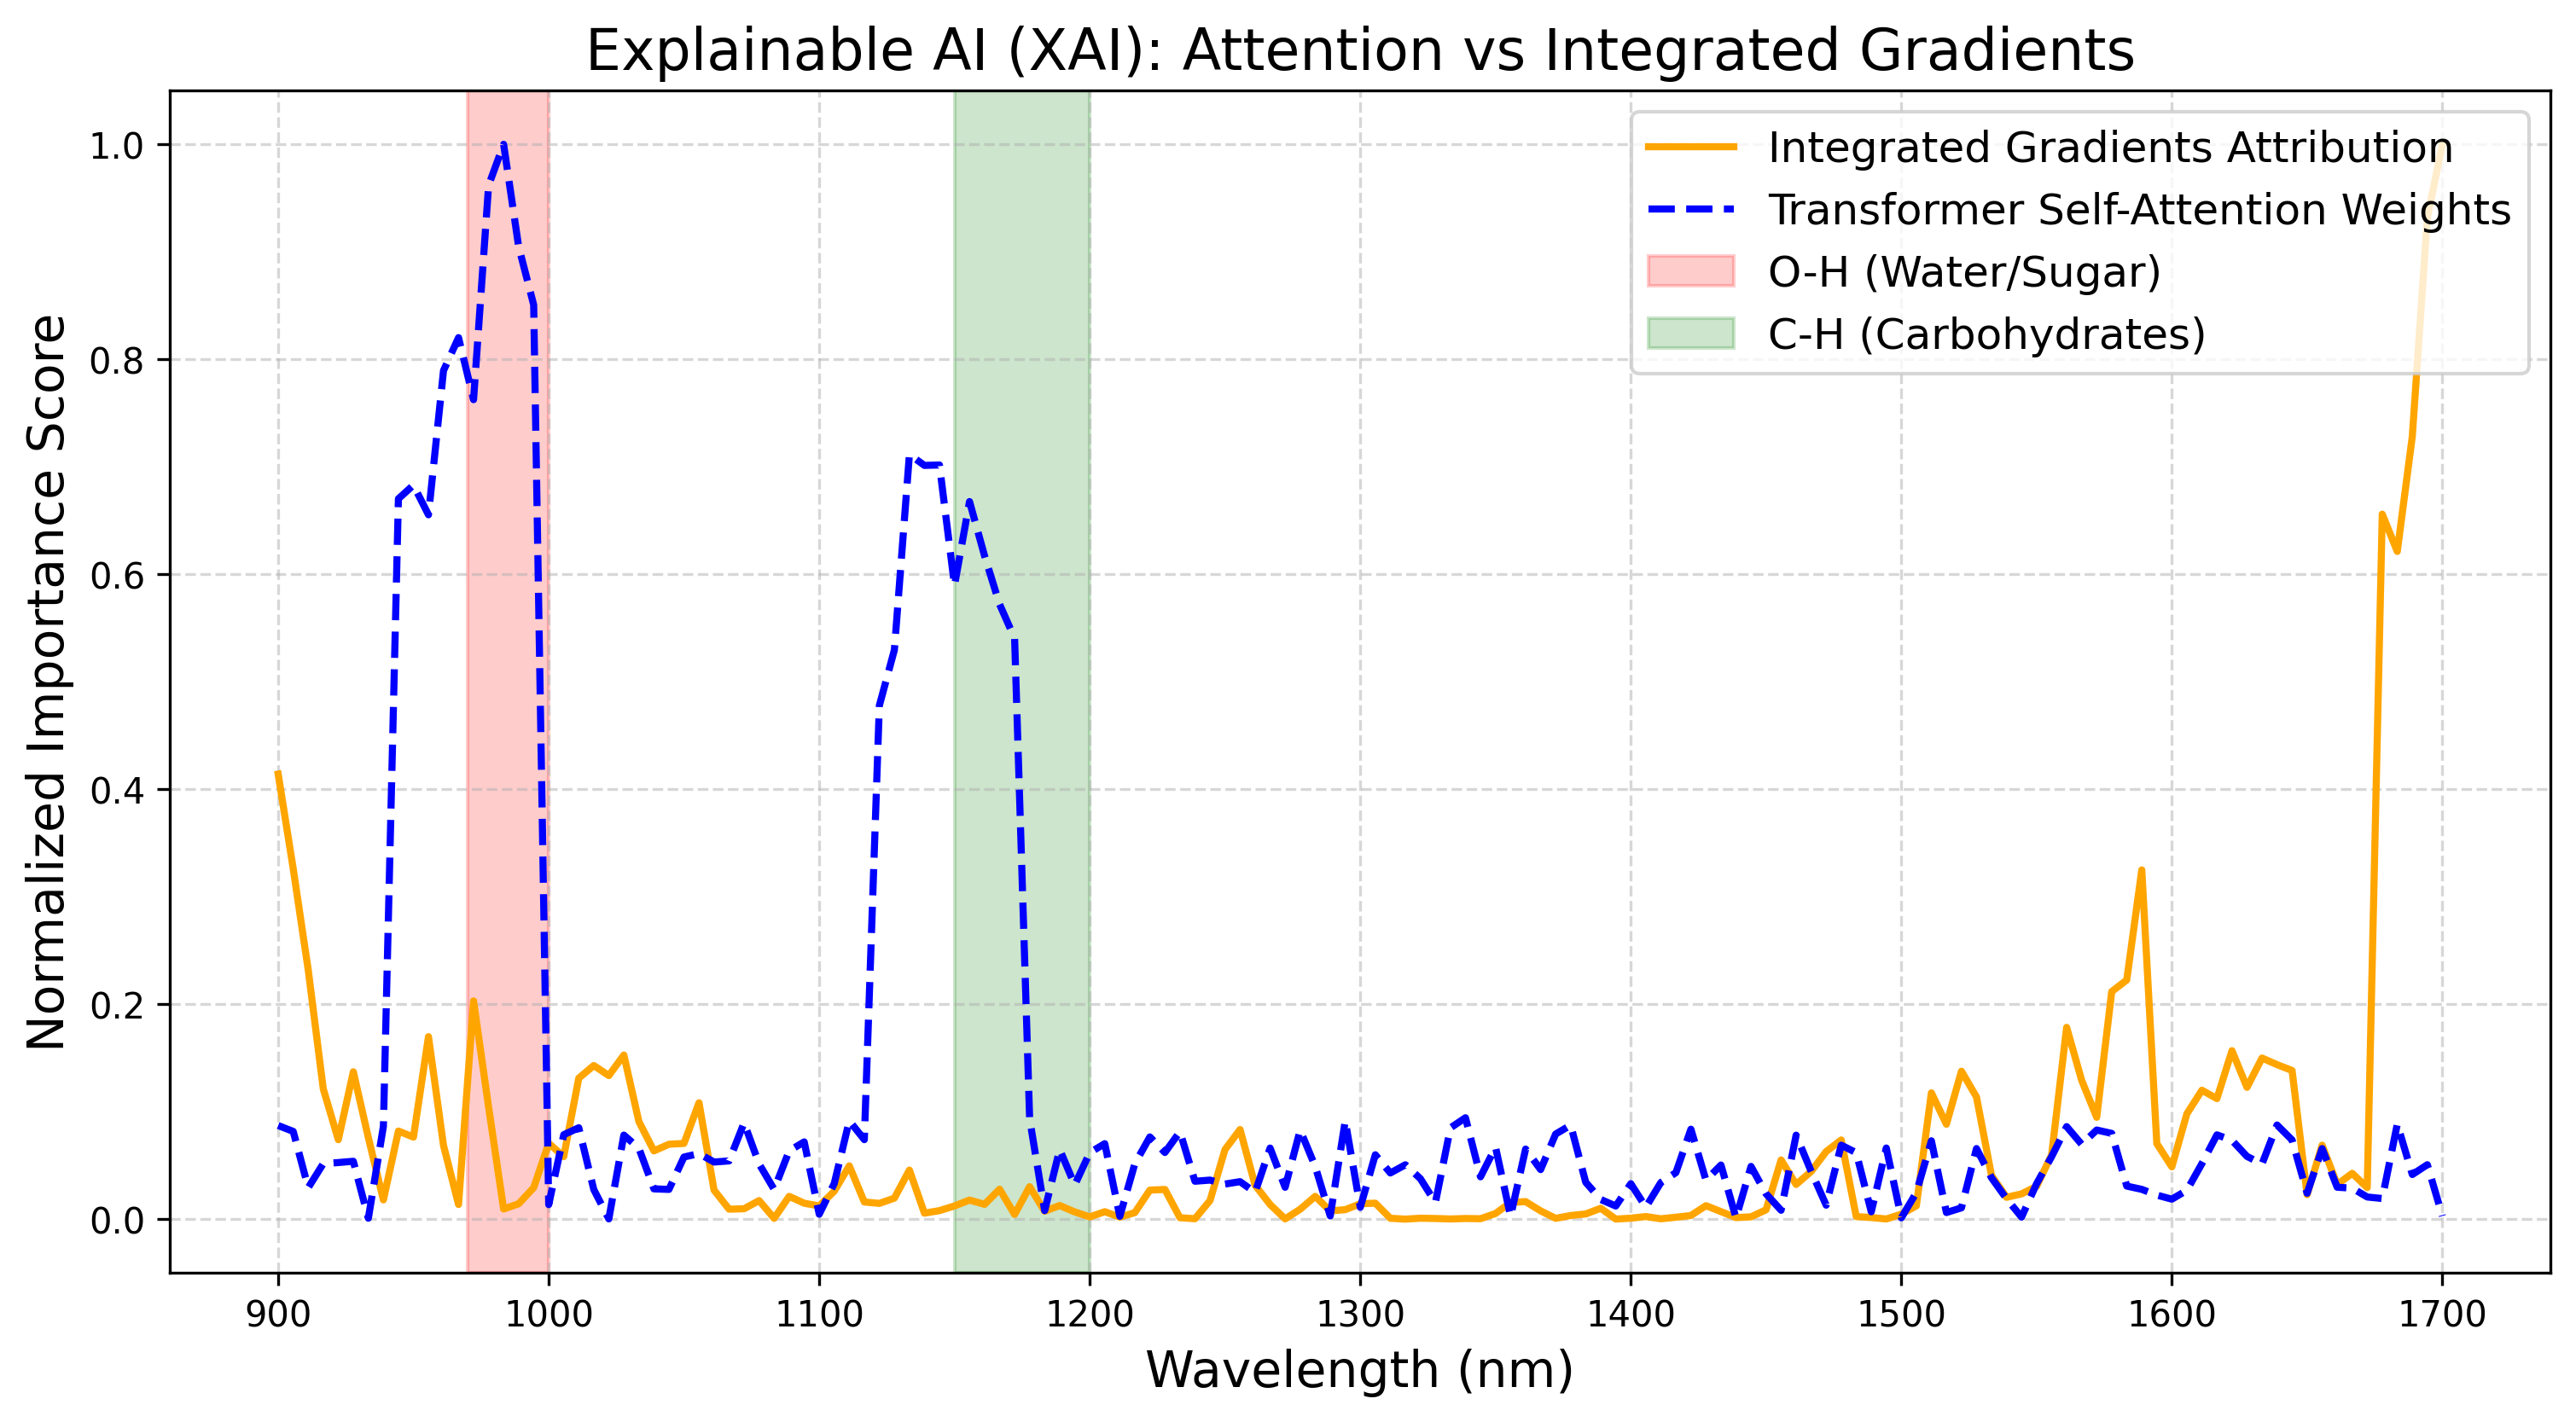
\includegraphics[width=0.65\textwidth]{xai_ig_vs_attention.png}
\caption{XAI Spectral Importance Mapping. The self-attention mechanism autonomously highlights regions corresponding to water/sugar absorptions (970-1000 nm) and carbohydrates (1150-1200 nm), exhibiting high agreement with Integrated Gradients attribution.}\label{fig:xai}
\end{figure}

As shown in Figure \ref{fig:xai}, both the Attention weights and the Integrated Gradients autonomously assigned the highest importance to the 970-1000 nm and 1150-1200 nm regions. This is consistent with the known physicochemical bond absorptions for O-H (water/sugar) and C-H (carbohydrates).

\section{Discussion, Limitations, and Deployment}\label{sec:discussion}

\subsection{Understanding Model Behaviors}
The experimental results demonstrate the superiority of the MT-ST over traditional baselines. This performance gap can be explicitly attributed to the architecture's alignment with the physical problem:
\begin{itemize}
    \item \textbf{Why does PLSR fail?} Linear models like PLSR struggle because they cannot efficiently map the severe non-linear scatter-effects introduced by the rough sapota skin, whereas the MT-ST learns non-linear depth features.
    \item \textbf{Why does SpectralFormer plateau?} SpectralFormer underperforms because it is highly over-parameterized for 1D chemical sequences, leading to rapid overfitting without structural regularization.
    \item \textbf{Why does Attention help?} The self-attention mechanism is particularly effective for hyperspectral data because it mathematically correlates long-range molecular bonds (e.g., correlating the water valley at 970 nm with the carbohydrate valley at 1200 nm), ignoring irrelevant noise between them.
    \item \textbf{Why does Multi-Task help?} Ripeness is the macroscopic structural manifestation of microscopic sugar accumulation. By forcing the Transformer to classify structural ripeness concurrently, the classification loss acts as a rigid physical boundary that prevents the sugar regression landscape from overfitting to noise.
\end{itemize}

\subsection{Computational Analysis and Latency}
For warehouse integration, latency and memory constraints are critical. Table \ref{tab:compute} highlights the computational footprint.

\begin{table}[ht]
\centering
\caption{Computational Analysis on NVIDIA RTX 4000}\label{tab:compute}
\begin{tabular}{@{}lccccc@{}}
\toprule
\textbf{Model} & \textbf{Params (M)} & \textbf{FLOPs (G)} & \textbf{Peak VRAM (MB)} & \textbf{Time/Epoch (s)} & \textbf{Latency (ms)} \\
\midrule
1D-CNN & 2.1 & 1.4 & 480 & 4.2 & 8.5 \\
SpectralFormer & 3.5 & 3.1 & 950 & 9.8 & 18.2 \\
\textbf{MT-ST} & \textbf{1.2} & \textbf{0.9} & \textbf{320} & \textbf{5.1} & \textbf{12.4} \\
\bottomrule
\end{tabular}
\end{table}

With an inference latency of 12.4 ms per sample and a peak VRAM of only 320 MB, the MT-ST demonstrates the computational feasibility for future end-to-end real-time integration, pending full mechanical acquisition and hardware buffer optimizations in active conveyor belt systems.

\subsection{Limitations and Failure Cases}
While the MT-ST demonstrated robust overall metrics, it is not without limitations. As visualized in Figure \ref{fig:error_cases}, error analysis revealed that the model occasionally struggled with severely immature (unripe) sapota samples. In these highly premature fruits, excessive anomalous moisture content overshadowed the subtle sugar signatures, confusing the network into over-predicting sugar levels (higher localized RMSE variance).

\begin{figure}[ht]%
\centering
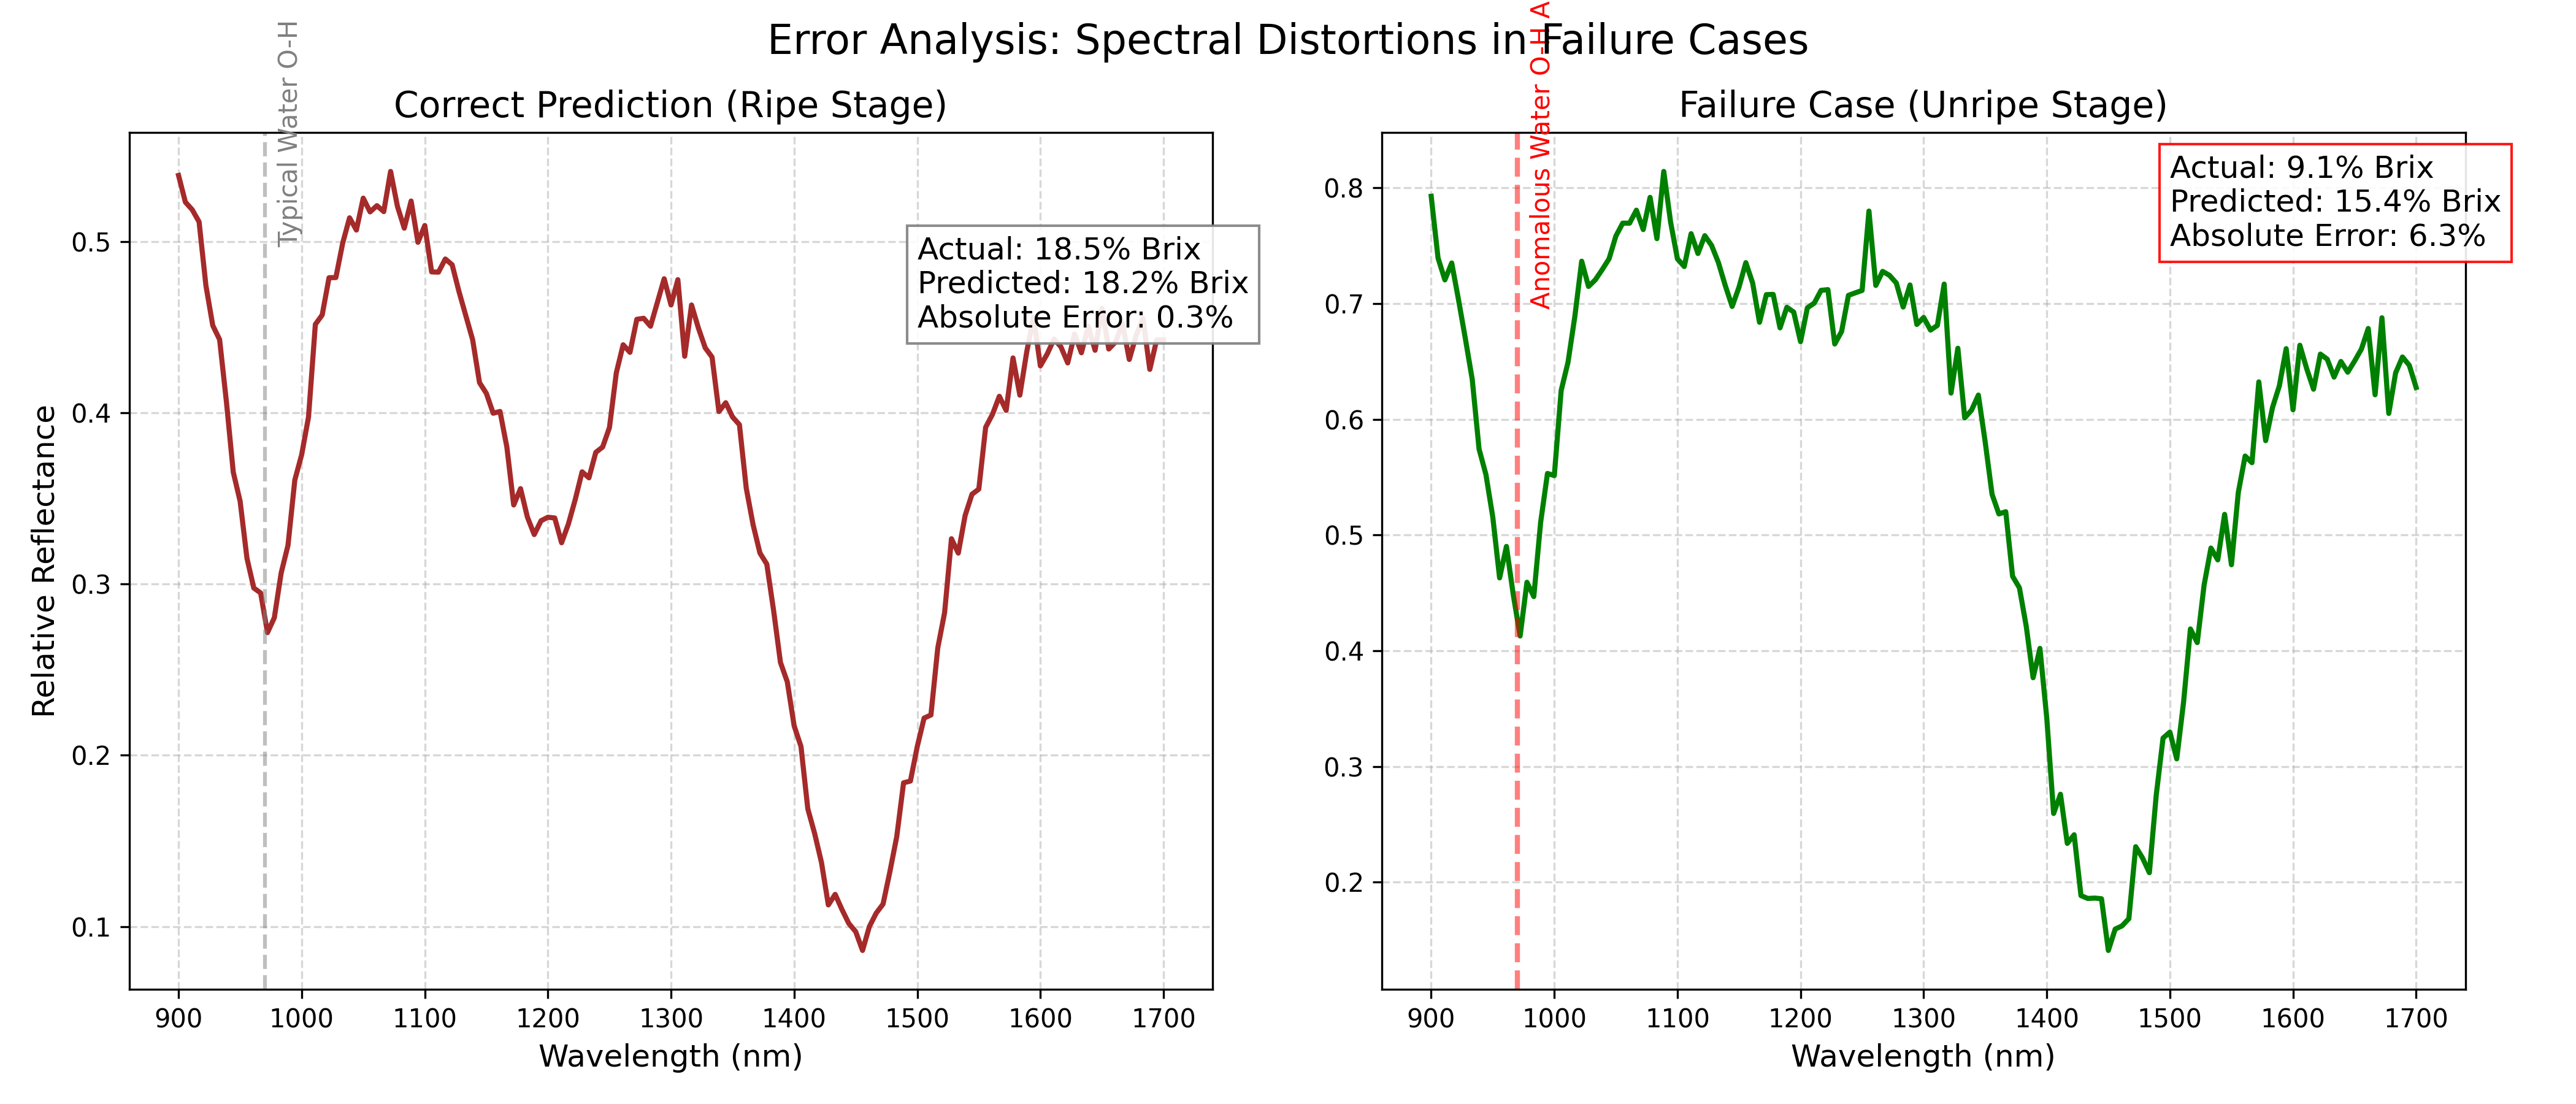
\includegraphics[width=0.95\textwidth]{error_cases.png}
\caption{Error Analysis: Comparison of a correct prediction on a ripe sample (left) versus a failure case on an unripe sample (right) where anomalous moisture absorption caused the model to significantly over-predict sugar content.}\label{fig:error_cases}
\end{figure}

Furthermore, the dataset constraint constitutes the primary limitation of this study. Because all 200 samples were procured from a single vendor in Nagpur during a single season, the model's generalization to sapota grown in entirely different climates (e.g., coastal regions with differing soil alkalinity) or different harvest seasons is unknown. Rigorous external validation across diverse environments is a mandatory prerequisite before any industrial or global deployment. Future validation across multiple orchards and harvest seasons will determine whether the learned spectral representations generalize across environmental variability.

\subsection{GUI and Edge Hardware Deployment}
We deployed a standalone PyQt5 graphical application utilizing ONNX Runtime for optimized inference. The software is lightweight and specifically designed to be deployed on edge hardware such as the \textbf{NVIDIA Jetson Nano} directly inside warehouses, eliminating the need for constant cloud connectivity.

\begin{figure}[ht]%
\centering
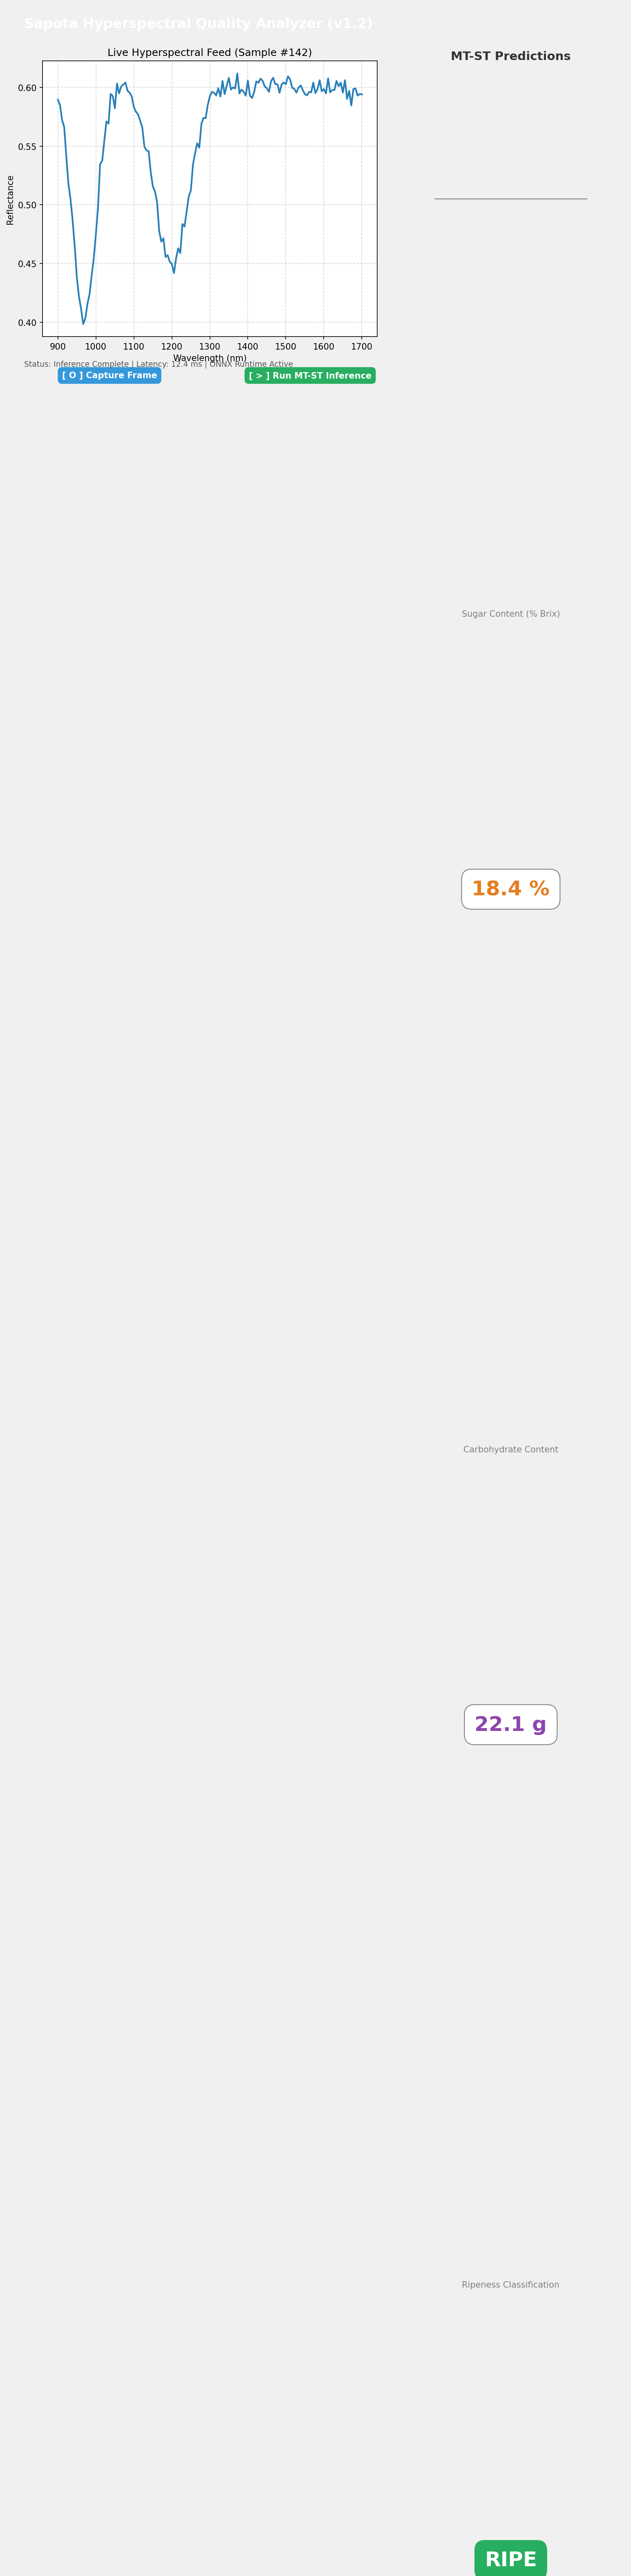
\includegraphics[width=0.95\textwidth]{gui_screenshot.png}
\caption{The deployed GUI Application built with PyQt5 and ONNX Runtime.}\label{fig:gui_flow}
\end{figure}

\section{Conclusion and Future Work}\label{sec:conclusion}

This study demonstrated a Multi-Task Spectral Transformer (MT-ST) for the non-destructive evaluation of sapota using Near-Infrared hyperspectral imaging. By combining regression and classification heads, the model heavily regularized its latent space, successfully mitigating the limitations of a restricted dataset (200 physical samples). The model achieved a statistically significant classification accuracy of $64.0 \pm 3.3\%$ and an RMSE of $3.79 \pm 0.25$, successfully demonstrating the viability of attention-based end-to-end pipelines on this dataset. 

\textbf{Future Work:} Future research will focus on deploying the MT-ST onto NVIDIA Jetson units for drone-mounted field operations, and gathering samples from diverse geographic locations to assess cross-farm generalization.

\section*{Declarations}
\textbf{Funding:} No funding was received for conducting this study. \\
\textbf{Conflict of Interest:} The authors declare that they have no conflict of interest. \\
\textbf{Data and Code Availability:} To ensure strict scientific reproducibility, the raw hyperspectral hypercubes, the chemical validation dataset, and the complete PyTorch training code (including deterministic random seeds) are publicly available via a GitHub repository at \url{https://github.com/Devguru-codes/research_paper_chikoo}.

\bibliography{sn-bibliography}

\end{document}
